


\section{Questions}

How do we model the constraints?

\subsection{Using full models}
I have implemented an algorithm that uses higher order models to approximate the constraints.

In this algorithm, we add additional degrees of freedom to the constraints to cut off points that have been evaluated and are infeasible.
The models are forced to be a given negative value at these points.

One question for this method is how many constraints to model.


I implemented Kriging, as this can use as many points as are available.
However, this requires using some artificial value of the constraints at infeasible points.

\subsection{Using linear models}

Another method is to add additional linear constraints each time a new point is evaluated and infeasible.

Each new linear constraint cuts off an infeasible point and stays atleast a fraction of the trust region away from that infeasible point.


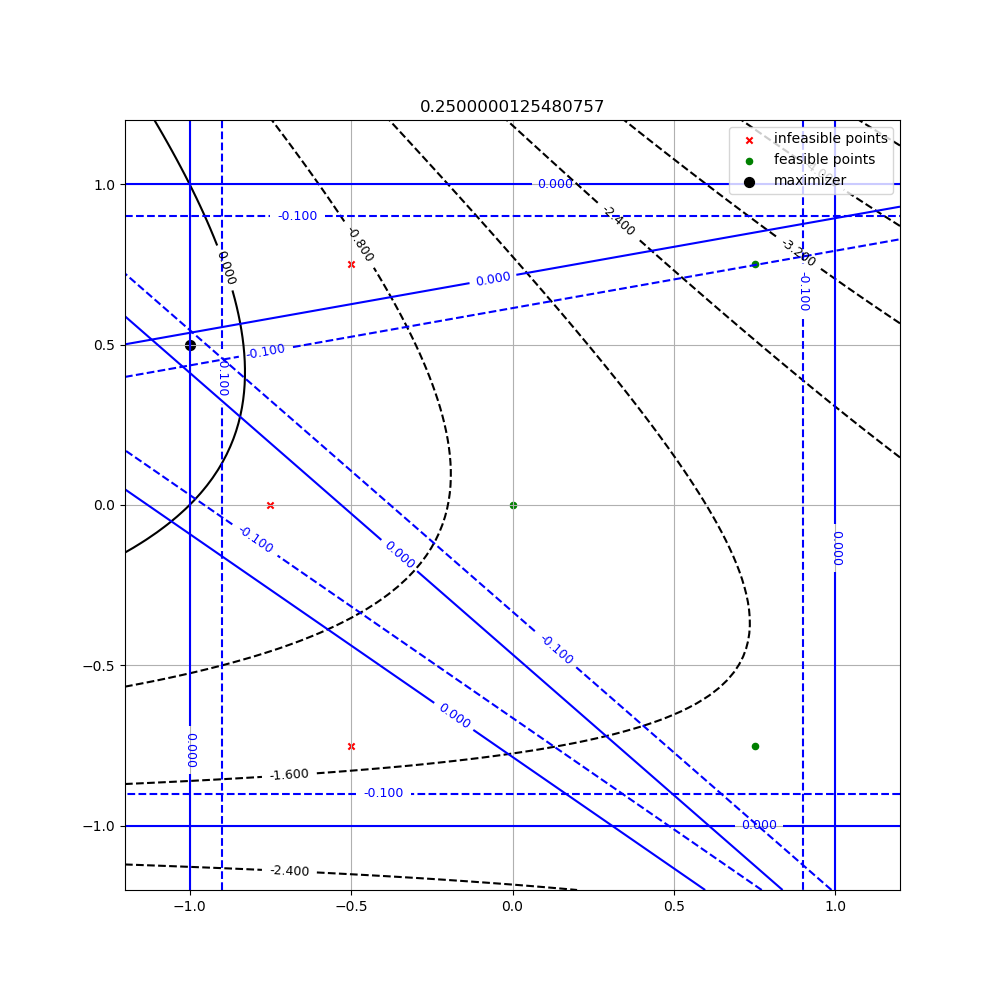
\includegraphics[width=300px]{images/pyomo_cut_solution.png}

\subsubsection{formulation}

The optimization program for finding this constraint is given by:

A set of $u^i, 1 \le i \le n_{I}$ infeasible points.
A set of $v^i, 1 \le i \le n_{F}$ feasible points.

The current Lagrange polynomial $\frac 1 2 x^T Q x + b^Tx$.
Require all infeasible point to be a distance at least $d$ from the feasible region.


Find a set of planes $(n^i, b^i), 1 \le i \le n_{P}$.

Require $n_P \ge n_I$.


What we want big:
\begin{align}
\max_{x} & \frac 1 2 x^T Q x + b^Tx &\\
 & {n^i}^T x \le b^i & \forall 1 \le i \le n_{P} \\
 & {n^i}^T v_j \le b^i & \forall 1 \le i \le n_{P}, 1\le j\le  n_{F} \\
 & {n^i}^T u_i \ge b^i + d & \forall 1 \le i \le n_{I} \\
 & \| n^i \| = 1 & \forall 1 \le i \le n_{I} \\
 & 0 \le x_i \le 1 & \forall 1 \le i \le n \\
\end{align}


A set of $v_i, 1 \le i \le n_{I}$ feasible points.




\subsection{Using a sacred region}

Another approach is to ensure that we will always have a large enough feasible region within the current trust region.

\begin{align*}
\max_{t \in \mathbb R, c \in \mathbb R^n} t \\
\| \xk - c\| \le t \\
\| {x_{inf}}_i - c \| \ge t \quad \forall i
\end{align*}

